\chapter{System Analysis Method}

\section{Introduction and Preliminaries}

The goal of this study is to develop a first experimental methodology intended to observe emergence-related aspects coming from the interaction of a Control System and a System Supervisor, analyzing the system in a \textsl{simulated} environment.\newline
The software architecture of an AV was simplified in two main components:

\begin{itemize}
	\item A \textsl{Controller}: a Neural Network trained with \textsl{reinforcement learning} algorithms to drive the car
	\item A \textsl{Safety Monitor}: a submodule of the System Supervisor, that checks whether the car is going too fast towards an object, processing data received from a LiDAR sensor, and if that's so, apply an emergency-brake
\end{itemize}

This work focuses on exploring the topic from a different point of view and to assess its \textsl{feasibility} in an experimental, simulated environment. Due to the system being composed by two constituent systems: the Controller and the Monitor, we think that a point of view based on the emergent behaviour resulting from the interaction of these systems can improve the quality of the assessment.

In this chapter is presented and discussed a method to study the safety level of an autonomous car over time, observing the emergence resulting from the interactions of a neural network controller and a safety monitor in a simulated environment.

The proposed framework is designed with particular attention on studying the emergence resulting from the interaction of these two Consitutent Systems.

The main aspects we are interested in this first stage of exploration are:

\begin{itemize}
	\item How the effectiveness of a monitor evolves when the neural network is learning
	\item Effects of training strategies on the effectiveness of a safety monitor
\end{itemize}

One of the most appealing features of neural networks is that they can be \textsl{trained} on data sets to improve their performance. One stage of training is done by collecting data over \textsl{n} steps and updating the weights of the prediction function. The weights of the function after $i$ training stages represents the \textsl{state} of the network at \textbf{epoch i}.\newline
A neural network will likely give good results after "enough" epochs. The harder the task, the more epochs are needed. Driving a car is a quite hard task and it's inimmaginable to save the weights of each epoch. Therefore, given a neural network N, we define a \textbf{checkpoint} as a generic epoch of N. Say we trained N for 1000 epochs. If we save the weights of the prediction function every 100 epochs, we will end up with 10 checkpoints:

\begin{center}
	$checkpoint_{1}\: <\: checkpoint_{2}\: <\: \dots \:<\: checkpoint_{10}$
\end{center}

where $checkpoint_{1}$ contains the network's weights at epoch 100, $checkpoint_{2}$ at epoch 200 and so on.\newline

Let's now consider a self-driving car that is being tested on the road (either real, or simulated). Its task is to ride the car the longest possible, without crashing. During the ride, the environment surrounding the car will change as it procedes in its run. It may happen that in some of the system's state, the probability of a subsequent crash becomes very high, like a pedestrian suddenly crossing the road: if and only if the action taken by the Controller will result in the pedestrian getting hit we will address it as a failure (of the controller). The same reasoning applies if the pedestrian is actually detected, and the car hits something else while trying to prevent it:

\begin{itemize}
	\item If the Controller takes \textsl{any} action that would result in a crash, it's considered failed
	\item If a hazardous event happens, i.e. a situation in which the probability of observing a crash is higher than usual, the Controller is considered failed if and only if its actions will not avoid the imminent failure
\end{itemize}

In this sense, at this stage of the work, we don't distinguish between changes in the environment that raises the probability of a crash (e.g. a pedestrian crossing the street) and hazardous actions take by the Controller (e.g. a sudden steer towards a wall).

If the controller fails in the way just described, it's the Monitor's duty to run a safety-routine in order to prevent the imminent system failure.\newline

In the case of a failure of the Controller, the Monitor not only needs to detect whether it failed or not, but it also must run a safety-routine to prevent a failure of the whole system. In this first phase of analysis, we consider the action taken by the Monitor to be always safe. This means that:

\begin{itemize}
	\item If the Monitor executes \textbf{all} the steps in the safety-routine, the system will be in a safe-state.
	\item A failure of the Safety Monitor may be one of the following:
	\begin{itemize}
		\item[1)] The obstacle is not detected
		\item[2)] The obstacle is detected but the routine fails to terminate its execution (i.e. the detection was too late)
	\end{itemize}
\end{itemize}

We consider the system failed if and only if both the Controller and the Safety-Monitor failed, as described above, leading to a crash.
With this scheme in mind, the states space for this system can be modeled as in figure 10.\newline

\begin{figure}[h!]
	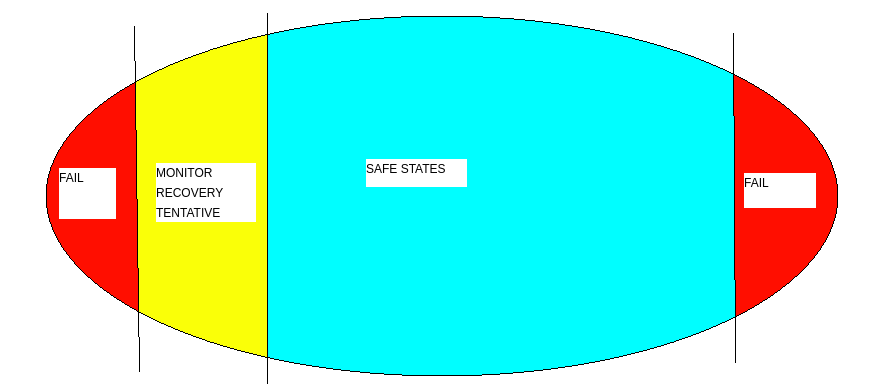
\includegraphics[width=\textwidth]{img/state-space-true.png}
	\caption{Representation of the system's states space}
\end{figure}

Based on our definition, we can divide the system states in 3 sets:

\begin{itemize}
	\item Safe States: states in which the Controller doesn't need an intervention of the Monitor
	\item Alert States: states in which the Monitor is required to intervene. A correct detection (and prevention) of the potential accident would result in a transition to the safe states space again
	\item Failure States: states in which an accident happened. It is important to notice that \textbf{not} all the situations can be detected by the Monitor. There are accidents that can not be prevented at all, in which no Monitor could save the system, therefore there is a direct transition from a \textsl{safe state} to a \textsl{failure state}
\end{itemize}


At the system level, we are interested in observing the probability of having a failure (crash) and how to minimize it. At the same time we want to observe how the effectiveness of the Safety Monitor changes when the Controller is trained over time.

In order to achieve this, $m$ checkpoints are saved for later testing and comparison. This is useful not only for checking that the network is improving during the training, but also to have a better understanding on how useful is the Monitor when the Controller becomes more and more expert. This is mandatory for the experimental activity, as different checkpoints of the same network are tested under the same identical conditions, to observe how the behaviour of the Controller changes over the training activity.

The need for multiple checkpoints is mandatory not only to test that the network is improving, but also to observe how the monitor's effectiveness changes over time. Moreover, if many checkpoints of the same network are tested in the same scenarios, it is possible to extract interesting measures and compare the behaviour of 2 checkpoints in the same situation, as we'll see in the next section.

Before the analysis can start, $n_{h}$ scenarios must be defined. A \textsl{Scenario} is a set of initial conditions (e.g. the spawn point of the car, seeds used in random number generators$\dots$) in which the car is intended to be tested. The pedix $h$ represents the difficulty level for the specific case. The purpose of this is that we are interested in testing the car under the same initial conditions, except for one factor, in order to have a better understanding on what makes the system fail more often. The $h$ variations should be developed with growing difficulty and at the same time they must be realistic. Given a Scenario $S$, examples of variations may be: to increase the number of cars in the scenario, or to simulate adversal weather conditions. A combination of these 2 variations should result in a \textsl{harder} variation of the scenario\footnote{It is important to point that what we think to be "harder", may in reality be easier to handle for the car.}. It's important to keep in mind that these scenarios, once defined, should not be changed as they will be used for testing all the checkpoints. A change in the settings of a scenario (except for variations) should be considered as a new one.

We hope that the results collected here will help in the process of understanding what makes a situation \textsl{"harder"} than others for such systems.

\section{Experimental Method}

The approach used for this exploratory work is divided in 3 phases:

\begin{itemize}
	\item Phase 1: Given $c$ checkpoints of a neural network and $n_{h}$ scenarios, the Controller is tested in all the scenarios and its runs are recorded
	\item Phase 2: The Monitor is tested by \textsl{repeating} the runs recorded in phase 1, attaching the Safety Monitor to the system
	\item Phase 3: The network is retrained from the last checkpoint recorded, using different strategies to improve its performances. The new Controllers obtained and the (same) Safety Monitor are then retested in all the $n_{h}$ scenarios
\end{itemize}


In the first phase we are interested in assessing the goodness of the neural network and of the Monitor. This is done in 2 different steps. 

In the first step, the $m$ checkpoints of the Controller are tested in all the scenarios. In this step we are mostly interested in observing how the \textsl{Reliability} of the Controller changes with respect to these checkpoints.

One of the main problems when testing a neural network is that of \textsl{repeatability}. It is very unlikely that the \textbf{same} neural network, under the \textbf{same} initial conditions, will behave in the same manner in multiple runs. Due to this property of networks, it may happen that the failure mode observed in one of the runs of the scenario $s_{i}$ will never happen again, or the time needed to make it happen again may be very long.
How the scenarios and their variations are created is fundamental to observe specific failures, however it's impossible to think to \textsl{all} the possible failure situations that may happen, for this reason we think that the scenario-variation approach may help in solving this issue, creating harder operational situations in which the factors that lead to a crash may be studied.

The repeatibility issue was solved by creating a \textsl{black box} for each run of the scenarios developed for testing. This approach is used to keep a trace of the Controller's actions, so that the specific run may be studied more fully to understand what made tha Controller fail. These data can be then used to better study what hazardous situations are covered by the Controller at a specific checkpoint $j$, and if these situations are still covered when the network is tested at the checkpoint $j+x$.\newline


\subsection{Controller Testing}

The Controller is tested in isolation in each scenario, for each difficulty level, until a crash occurs. The situation in which no failure is recorded is still a possibility (even if the difficulty level somehow mitigates this issue). A reasonable alting criteria is out of the scope of this work and is still a problem in the academic community, however, as noted in the previous section, this problem may be solved.\cite{zhaoStrigini}

The reasoning behind the choice of isolating the in order to test it Controller, comes from some of the problems issued during the method development phase.
The main problems are the \textsl{repeatibility} and \textsl{non-intrusiveness}. As pointed before, the \textsl{repeatibility} issue for the neural network is solved by creating a \textsl{black box} containing informations about the car's state in each frame. At the same time we can not think about testing the whole system at once (Controller \textsl{and} Monitor) because a safety-brake executed by the monitor will most likely change the environmental conditions for the rest of the simulation and we would not be able to compute measures about the goodness of the Controller itself. Testing the Controller in isolation helps to solve these issues and it's preparatory to the second phase.

Recording the actions taken by the Controller for \textsl{each} frame (as well as other measures such as the vehicle's speed in that frame) make it possible to have a great control over the data, as a single run may be repeated many times to gather additional data if needed.

When the controller has been tested for each difficulty, in all the scenarios at least the followings must be computed:

\begin{itemize}
	\item $MDBF_{i,j} = \frac{\#\: of\: faults}{meters\: travelled}$
	\begin{itemize}
		\item[-] Mean Distance Between Failure for the $i^{th}$ checkpoint, at the $j^{th}$ level of difficulty
	\end{itemize}
	\item $MTBF_{i,j}\: =\: \frac{\#\: of\: faults}{operational\: time}$
		\begin{itemize}
		\item[-] Mean Time Between Failure for the $i^{th}$ checkpoint, at the $j^{th}$ level of difficulty
	\end{itemize}
	\item $FR_{i,j}\: =\: \frac{1}{MTBF_{i,j}}$
	\begin{itemize}
		\item Failure Rate of the $i^{th}$ checkpoint at the $j^{th}$ level of difficulty
	\end{itemize}
	\item $R_{i,j}(t)\: =\: e^{-FR_{i,j}\cdot t}$
	\begin{itemize}
		\item Reliability Function of the $i^{th}$ checkpoint at the $j^{th}$ level of difficulty, i.e. the probability that the Controller $C_{i}$ is not failed at time $t$ when operating at difficult $j$
	\end{itemize}
	
	\item[-] All these measures are aggregated to compute overall performance metrics of a Controller $i$, without being specific to the difficulty level, but still computed separately for deeper examination of the Controller's behaviour in different environmental conditions
	
\end{itemize}

When measuring the reliability function $R(t)$ of a system, one of the main measure of interest is its Mean Time To Failure, because it is easy to compute in simulated environments, and it's used to compute the rate $\lambda$ of the exponential function.
In the Automotive Sector however, data are usually computed with respect to the travelled distance, i.e. Mean Distance to Failure, rate of crashes per kilometers, and so on.
With our approach, if the simulated environment and the hardware running the simulations are powerful enough to run the simulations at a fixed time-step, it's very easy to switch the point of view on the data.

As long as the neural network is trained properly, we expect the following disequation to hold: $R_{i}(t)\: \leq \: R_{j}(t)$, where $i$ and $j$ are 2 checkpoints, with $i\: <\: j$. This can be easily verified using the approach defined above to collect the data.

\begin{figure}[h!]
	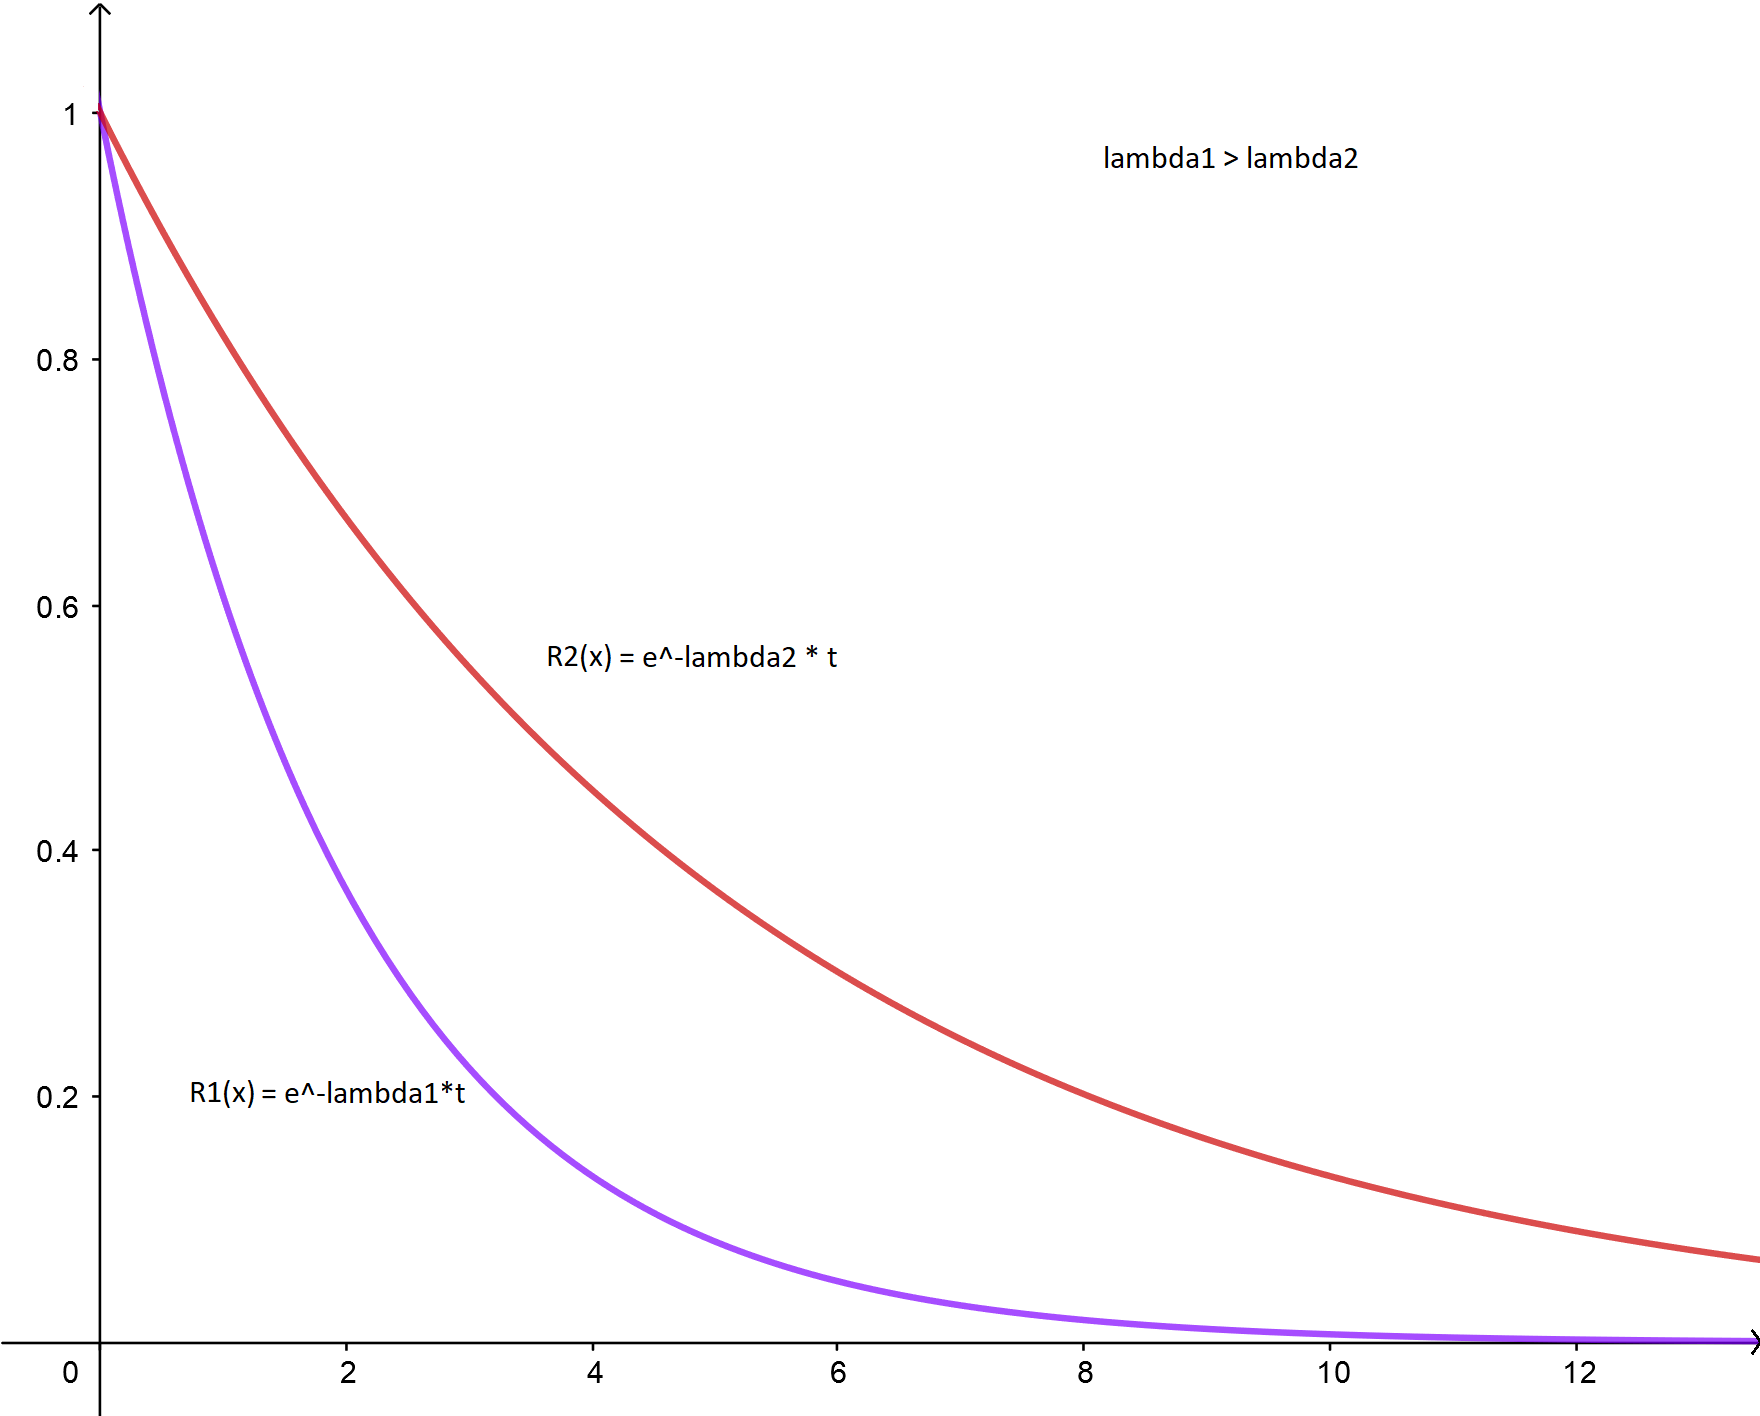
\includegraphics[width=\textwidth]{img/reliability-curve.png}
	\caption{The Reliability function measures the probability that at time $t$ the system is still operating. We expect that more expert drivers (i.e. more trained networks) are capable of longer runs than little trained networks}
\end{figure}

\vspace{0.8cm}

If the Simulator used for testing allows it, other data should be recorded too, in order to enhance the comprehension of the Controller's behaviour, such as:

\begin{itemize}
	\item The car's instantaneous speed and acceleration vector at each frame
	\item With \textsl{what} the car crashed (e.g. a vehicle, a pedestrian, a generic obstacle$\dots$)
	\item Define one or more \textsl{destination goal(s)} and record whether the vehicle reached it or not
	\item Environmental conditions at time $t-x$, if a crash occurred at time $t$ 
\end{itemize}

These data are fundamental to distinguish between \textsl{"safe"} and \textsl{"catastrophic"} failures. For example, if a fence is hit at a speed, let's say, less than 10km/h, it may be flagged as a less serious crash than hitting a pedestrian at the same speed.

As the Controller learns, we expect the \textsl{Reliability Function} and the \textsl{MTBF/MDBF} to increase, since a trained driver should in principle cause less crashes than a non-expert one, therefore increasing the value of the MTBF and possibly the y values of $R(t)$.

If the \textsl{black box} makes use of enhanced data (such as the ones listed above), it is also possible to observe changes in the car's behaviour with respect to the scenario and the difficulty level. For example: if we define a difficulty $k$ by doubling the number of cars in the scenarios, it may happen that it is observed an increasement on the amount of collisions against other obstacles. If that's so, the simulations should be studied more deeply to enforce the training strategy in a certain direction, as this may mean that the Controller is going to crash on walls while trying to avoid other vehicles.


\subsection{Monitor Testing}

Once the Controller's runs are recorded as described previously, the Monitor testing can start.

The goal of this phase is not only to see how good the Safety Monitor is in preventing crashes, we are also interested in observing evidences about which situations are \textsl{"hard"} for the Monitor, and which for the Controller. 

As the network becomes more expert, it may happen that its behaviour evolves in a way such that the Monitor is no more able to detect imminent failures, because the Controller is now good enough to cover all the failures previously covered by the Monitor, and the hazards caused by its novel behaviour are such that the Monitor is not able to detect them.

However, the opposite is also a concrete possibility. For example, in the first epochs the Controller may drive in a "crazy" manner, e.g. with a lot of sudden, high-angle steerings and riding at high speed. The Monitor will obviously have more problems in predicting what the next state will be due to the unpredictability of the Controller's behaviour. The more the network learns, the more it will (hopefully) ride smoothly, making it easier for the Monitor to detect possible, imminent crashes.

The main problem that should be addressed here is that the Monitor effectiveness may decrease, while the network is learning, resulting in a useless component that may even be detrimental to the system's \textsl{performability}: the Controller may become good enough to be able to cover all the hazardous events covered by the Monitor at an earlier checkpoint. This may not change the whole safety of the system, if we consider the actions taken by the Monitor as inconditionally safe, but it would result in lesser smooth rides, due to the safety-brakes applied by the Safety Monitor.\newline

The Monitor is tested as follows: the black boxes created during the Controller testing phase are used to \textsl{repeat} the runs. The initial conditions must be \textsl{identical} as well and should be saved as part of the black box in the previous stage. The runs of the Controller previously recorded are now repeated, attaching the Monitor to the System and recording the alarm raised during the run and if it was able to prevent the crash that originally occurred.

In this stage of the analysis, the major concern was that of \textsl{non-intrusiveness}. For the reasons pointed above, we can not think about rerunning the simulations just by attaching the Safety Monitor and watch how it goes. The Safety Monitor, by definition, \textsl{overwrites} the Controller's action if an alert is raised, changing the next part of the run. This is theoretically not a problem, if one can distinguish between false and true positives. However, we can not know in advance what a false positive will be without creating a software capable of sensing and mapping the environment. But this is a Safety Monitor itself and, as every tool of this kind, it will have false positives even if extremely low, therefore this approach can not solve the problem.

The idea is to record the alerts generated during the run, without enabling the safety-procedure (e.g. the brake). Since we are going to repeat exactly the runs recorded in phase 1, it's possible to know the instant of time $t$ in which the transition to the \textsl{alert state} before the crash occurred. With this information, all the alerts raised before $t$ are indeed false positives, or false alarms, since we know $t$. Enabling the Monitor to activate the safety-procedure after this instant of time, makes it possible to approximate its coverage. 

As pointed in the previous chapter, to measure how good a model is in classification problems, we observe its predicted values with respect to actual values, visualized using the confusion matrix. However, for \textsl{real time critical systems} it's not easy, if not impossible at all, to measure all of them. In particular, it's not always possible to understand when the Controller avoided a crash and the monitor \textsl{did not} raise an alarm. This makes very hard to measure the amount of true negatives because in most of the cases, this kind of situations may be seen only when a human operator analyse the specific run, introducing a level of arbitrariness when computing measures such as \textsl{true negatives}.

In particular, an input for the Safety Monitor is composed by multiple, timed inputs, that can be seen as the evolution of the environment while the system is performing its operations. For this reason, it is hard to understand whether the next state will be an alert or a safe state because we don't know \textsl{when} the series of inputs that will eventually result in a crash will begin.

This puts some limits on the metrics and the rates that can be computed for the Monitor as they require the amount of true negatives.

At the same time, the Safety-Monitor classifies the system's state \textsl{in each frame}, receiving LiDAR data, processing them, and deciding whether a safety-brake is needed or not. Following this reasoning, we can consider every frame in which the Monitor doesn't raise an alert as a \textsl{true negative}, due to the \textsl{real-timeness} of the System.
This approach allows us to compute all the measures usually defined for statistic classification models.\newline

Since the order of magnitude of \textsl{true negatives} is likely to be much bigger than the the other metrics, for the reason just described, we had to combine together true and false positives and negatives in order to have meaningful values, e.g. Precision and Accuracy. This is because false positive rate is expressed as $\frac{FP}{FP+TN}$, resulting in values with many zeroes before the first meaningful digit. Moreover, to provide an intuitive rate measure for false positives, it was decided to compute the amount of false positives over the distance travelled in a run.

The rates of correct/wrong Monitor's predictions were computed as defined in Chapter 2, and they can be used for the purpose of comparison among Checkpoints:

\begin{itemize}
	\item Sensitivity and Miss-Rate
	\item Specificity and Fall-out
	\item Accuracy
	\item Precision
	\item Matthew's Correlation Coefficient
	\item False Positives per Meter
	\item Precision-Recall Plot
\end{itemize}

\textsl{Accuracy} and \textsl{Precision} were chosen following an ISO standard. The concept of \textsl{Accuracy} is replaced by the \textsl{Trueness} of predictions, and \textsl{Accuracy} is defined as a description of the combination of \textsl{random} and \textsl{systematic} errors, hence requiring high accuracy and precision. \cite{isoacc}
Matthew's Correlation Coefficient is defined as the most informative metric to evaluate a \textsl{Confusion Matrix}, as it is computed as a combination of all the predictions (true and false positives and negatives) and it proved to give more accurate overall informations than $F_{\beta}$-score. The reason why we decided to don't consider $F_{\beta}$ is that, in general, it doesn't work well with unbalanced datasets providing results that are too optimistic or too pessimistic, based on the weight $\beta$. Due to the \textsl{huge} amount of \textsl{True Negatives} and since we are interested in the \textsl{overall} Monitor's effectiveness we decided to use $MCC$ as a measure of the Monitor's performances. \cite{mcc}
False Positives per Meter is used to estimate how the System would behave in a context where both the Controller and the Safety-Monitor are enabled and working together, estimating the amount of wrong safety-brakes applied by the latter.
Plotting the ROC\footnote{Receiver Operating Characteristic} Curve, a graphical plot used to visualize the diagnostic ability of a classifier tool, would have provided a mean to quickly visualize the Monitor's effectiveness, however this approach was not feasible. A ROC Curve is made by defining the x-axis by FPR, and the y-axis by TPR. The plot is then split by the line $y=x$: values over this line depicts the ability to identify positive cases as such, values under this line represents predictions worse than random predictions, while values on the line represents random predictions. Due to the high imbalancement of our dataset, where the false positive rate is likely going to get values lower than $10^{-2}$, due to how true negatives were defined, the plot would be flattened "on the left side".

For this reason, we decided to use the \textsl{Precision-Recall Curve} to provide a visualization mean, a curve obtained defining the x-axis by \textsl{Recall} (True Positive Rate) and the y-axis by \textsl{Precision}, using data collected for each Checkpoint in all the difficulties. Since the Monitor is just classifying states as \textsl{safe} or \textsl{hazardous} and this is done \textsl{real time} on data collected by the LiDAR sensor, we could not create a test-set to test the Monitor while changing the cut-off for deciding whether to brake or not and plot the whole curve. Therefore, \textsl{Precision} and \textsl{Recall} were computed in each level of difficulty, and these values were plotted to understand the correlation between level of difficulty and Monitor's effectiveness.\newline

When testing the Monitor, it is advisable to \textsl{"stress"} it under detrimental conditions, in order to collect more possible evidences and linkage among the data. Note that this aspect is independent from the \textsl{difficulty level} defined above, as it is something related to the environment itself that may give evidences about the \textsl{situations} in which the Monitor performs well, and those in which it doesn't (e.g. think about a LiDAR sensor in a very rainy environment: the observations will likely to be fuzzy/noisy) and it is more related to \textsl{fault injection} at a higher level.

The ways in which the parameters of a Safety Monitor can be tuned really depend on its implementation, and it's up to the developing team the decision on what and how many faults inject in the software. A very simple example can be that of reducing the amount of data read by the sensors (which will result in low-quality data and a poor mapping of the environment), or introduce some noise in the observations.

Doing this step when testing the Monitor allows also to understand how to tune the internal parameters of the software in order to have its \textsl{"best"} version, that will be used in the Controller retraining phase.

\subsection{Controller Retraining}

At this point we have collected data about the behaviours of the Monitor and the Controller. In this phase we are going to study how much this values vary with respect to the learning strategy adopted, when the neural network is retrained from the last checkpoint.

As said at the beginning of this chapter, we are considering a Controller composed by a neural network, trained with reinforcement learning techniques. These kind of algorithms make use of a \textsl{reward function} to tell to the network if it's behaving \textsl{"good"} (positive value) or \textsl{"bad"} (negative value) and it is calculated at each prediction step (i.e. at each action taken by the Controller).\newline

The training function needs the following parameters, that are recorded at each algorithm iteration:

\begin{itemize}
	\item[a)] Action taken by the Network
	\item[b)] State of the network in which the action was taken
	\item[c)] Reward given for the action taken in a certain state
\end{itemize}

In this phase we want to discover how training strategies for the neural network may affect the overall behaviour of the system, with particular attention on the effectiveness of the Safety Monitor.

To start an exploration in this topic, we defined 4 strategies and the outcomes we expect after the training is completed. These outcomes are \textsl{"forecasted"} in the sense that we don't know how the network will react to a change in the training strategy, nor if the observe behaviour will be the supposed one.

The strategies developed in this method are mostly based on the reward function and on the actions taken by the network:

\begin{itemize}
	\item[S1)] The reward function is now more punitive when the car hits something, while braking is slightly more rewarded, provided that the Car won't stop moving
	\item[S2)] The Safety Monitor is attached to the system and, if an alert is raised, the action of the network is replaced by the Monitor's action (the safety-brake)
	\item[S3)] The network's action is replaced by the monitor's if it raises an alert. The network is given a positive reward for behaving like the Monitor
	\item[S4)] The training step is stopped and the network is given a \textsl{negative} reward if an alert is raised
\end{itemize}

Using S1 we expect at least the Controller's mean time/distance between failures to be lower. Giving a more negative reward for collisions and a little positive reward for braking (if the car doesn't stop moving) should force the car to prefer a brake instead of a swerve (that could result in a \textsl{new} hazardous situation), therefore improving its time between failures and its travelled distance.

The purpose of S2 is to \textsl{"teach"} to the network to brake whenever an alarm is raised by the Monitor. A possible outcome is that the alert states previously covered by the Monitor become now safe states. However the Monitor's false positives will inevitably have an impact on the system's availability, caused by erroneous safety-brakes.

S3 is pretty much similar to S2. We expect that giving a positive reward when behaving like the Monitor may increase the learning speed.

S4 is the most promising strategy and it may give the most interesting results. Giving a negative reward and alting the training step when the Safety Monitor raises an alarm, regardless if it's a true or false positive, should force the network to completely \textsl{avoid} the situations in which the Monitor intervenes. Essentially we expect that the effectiveness of the safety component will be drastically reduced.\newline

After the four Controllers are trained enough, the new systems are tested as in phase one. The same measures listed before are approximated for the Controllers and the Monitor and the results are compared with the original checkpoints.

